\begin{frame}[parent={cmap:software-testing-foundations}, hasprev=false, hasnext=true]
\frametitle{Fases de teste}

\begin{block:fact}{O que devo testar primeiro?}
\begin{itemize}
	\item O que devo direcionar ao teste de software?

	\item A definição de um único alvo para cada atividade de teste é fundamental para teste de software sistemático.
	\begin{itemize}
		\item Fono na aplicação e restrição de técnicas disponíveis (diminuindo assim os custose, provavelmente, aumentando a eficácia).
	\end{itemize}

	\item Uma abordagem de senso comum seria iniciar o teste com a menor função possível, e depois prosseguir para testar as interações entre as funções e, finalmente, o sistema como um todo.
\end{itemize}
\end{block:fact}
\end{frame}


\begin{frame}[hasprev=true, hasnext=true]
\frametitle{Fases de teste}
\label{concept:fase-de-teste}
\label{concept:fase}

\begin{block:concept}{Definição}
A fase de teste é uma categorização da atividade de teste que está diretamente relacionada com o ciclo de vida do software e as atividades que acontecem no software.
\end{block:concept}

\begin{block:fact}{Definições}
\begin{itemize}
	\item Fases de teste permite que o dispositivo de teste se concentre em vários aspectos do software e utilize diferentes critérios de teste para cada um;

	\item As atividades de teste são organizadas em fases de teste de modo que o teste inicie com a menor unidade executável até alcançar o software como um todo:
	\begin{itemize}
		\item Teste de unidade;
		\item Teste de integração;
		\item Teste do sitema;
		\item Teste de aceitação.
	\end{itemize}
\end{itemize}
\end{block:fact}
\end{frame}


\begin{frame}[c]
\frametitle{Fases de teste}

\begin{block:fact}{}
    \centering
    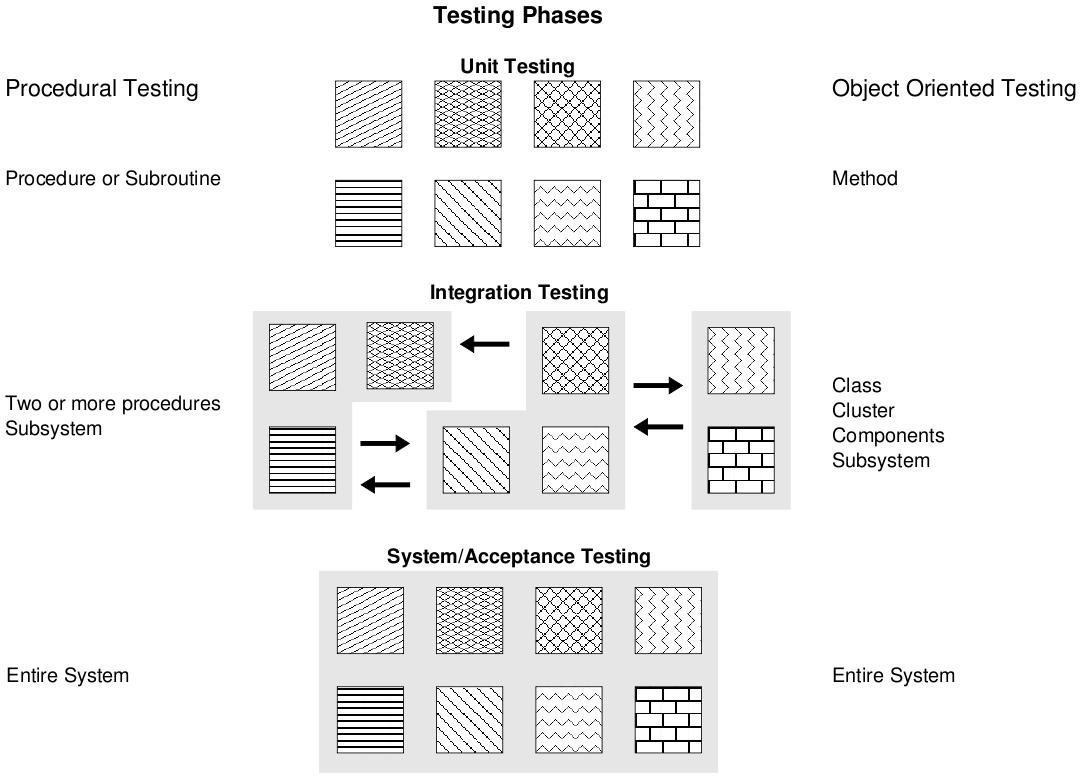
\includegraphics[scale=.3]{teste-de-software/conceitos-basicos/Imagens/fases-de-teste}
\end{block:fact}
\end{frame}


\begin{frame}
\frametitle{Fases de teste}
\framesubtitle{Teste de unidade}
\label{concept:teste-unitario}

\begin{block:concept}{Definição}
Teste de unidade verifica o funcionamento isolado de fragmentos do software que são testados separadamente.
\end{block:concept}

\begin{block:fact}{}
    \centering
    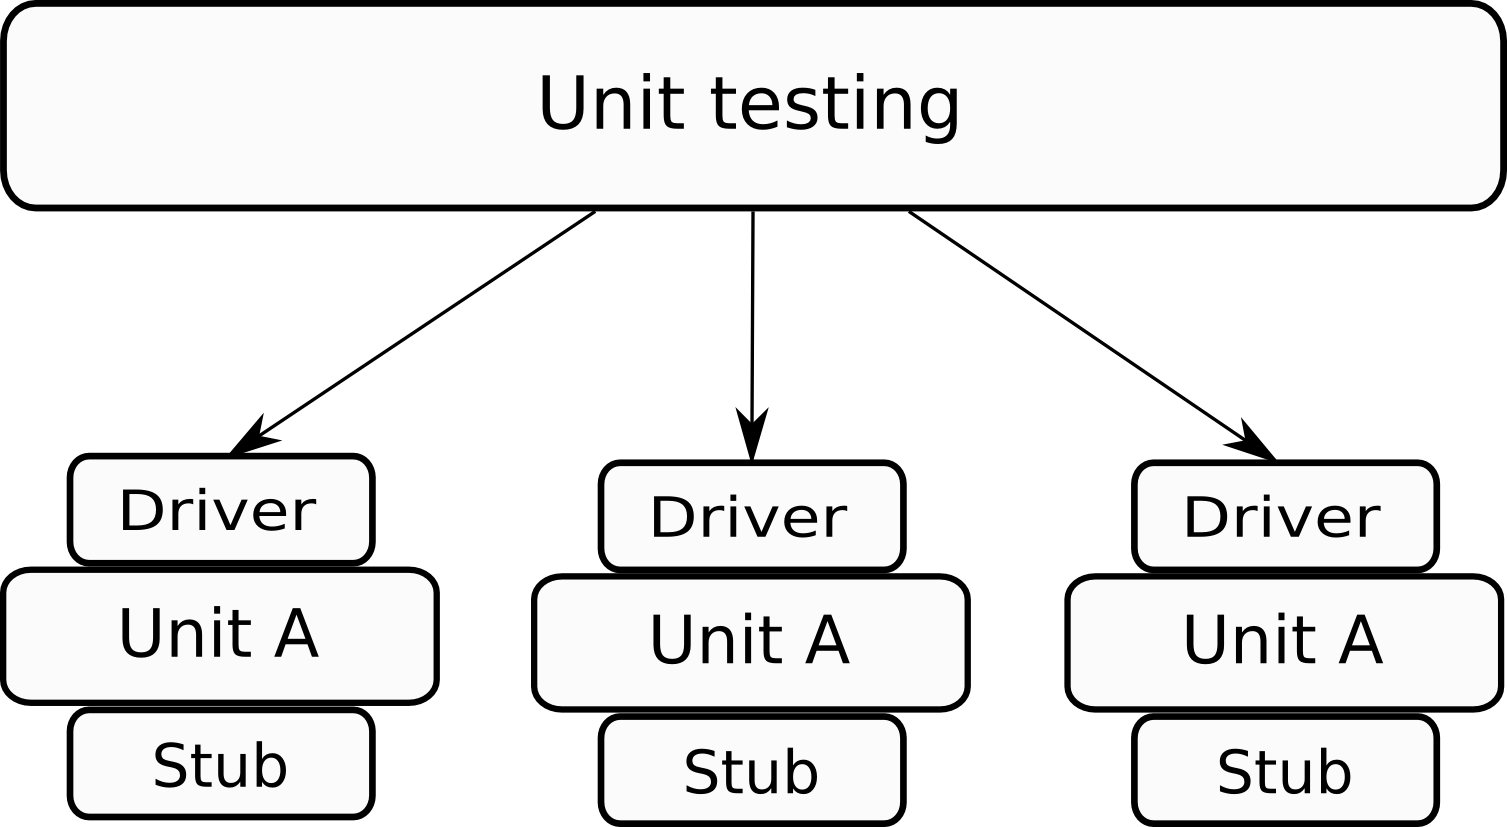
\includegraphics[width=5cm]{teste-de-software/conceitos-basicos/Imagens/teste-unitario}
\end{block:fact}

\hfill
\refie{example:pentium-fdiv-bug}{\beamerbutton{Example: Pentium FDIV bug}}
\end{frame}


\begin{frame}
\frametitle{Fases de teste}
\framesubtitle{Teste de unidade}

\begin{block:fact}{O que é uma unidade?}
\begin{itemize}
	\item Em teste de processo, a unidade é o procedimento ou a subrotina;

	\item Em teste orientado a objeto, a unidade é um método ou uma classe:
	\begin{itemize}
		\item Por enquanto, vamos considerar que a unidade é um método.
	\end{itemize}
\end{itemize}
\end{block:fact}
\end{frame}



\begin{frame}
\frametitle{Fases de teste}
\framesubtitle{Teste de unidade - Stubs}
  
\begin{block:fact}{Como testar uma unidade?}
\begin{itemize}
	\item Embora a definição diz para testar as unidades separademente, nem sempre isso é possível:
	\begin{itemize}
		\item Muitas unidade necessitam de dados de outras unidade.
	\end{itemize}

	\item A ligação entre os métodos é uma ameaça para o teste unitário. Assim, é desejável substituir algumas unidades por outras mais simples e previsíveis (apenas para o fim do teste de software).
\end{itemize}
\end{block:fact}
\end{frame}



\begin{frame}
\frametitle{Fases de teste}
\framesubtitle{Stubs}
\label{concept:stub}

\begin{block:concept}{Definição}
Um stub é uma unidade que substitui outra unidade utilizada pela unidade em teste.
\end{block:concept}

\begin{block:fact}{Por que devemos usar um stub?}
\begin{itemize}
	\item Stubs simula o comportamento de outra unida que ainda não foi implementado, mas foi chamado pela unidade em teste.

	\item Geralmente, um stub  simula o comportamento esperado da unidade utilizada com o mínimo de esforço computacional possível ou manipulação de dados.
\end{itemize}
\end{block:fact}

\hfill
\refie{example:stub}{\beamerbutton{Example: Stub}}
\end{frame}


\begin{frame}
\frametitle{Fases de teste}
\framesubtitle{Teste de unidade - Driver}

\begin{block:fact}{Como testar uma unidade?}
\begin{itemize}
	\item Mesmo que stubs pode ser usado para substituir unidades complexas para uma determinada unidade em fase de testes 
\end{itemize}
\end{block:fact}
\end{frame}



\begin{frame}
\frametitle{Fases de teste}
\framesubtitle{Teste de unidade - Driver}
\label{concept:driver}
\label{concept:test-driver}

\begin{block:concept}{Definição}
Driver é o software responsável por coordenar o teste de uma unidade.
\end{block:concept}

\begin{block:fact}{O que um driver faz?}
\begin{itemize}
	\item Drivers são usados para testar uma unidade que requer dados de entrada fornecidos por outra unidade:
	\begin{enumerate}
		\item Reúne os dados fornecidos pelo verificador;
		\item É passado para a unidade em teste na forma de argumentos;
		\item Que recolhe os resultados produzidos pela unidade, e;
		\item Mostra todos eles para o verificador.
	\end{enumerate}
\end{itemize}
\end{block:fact}
\end{frame}


\begin{frame}[c]
\frametitle{Fases de teste}
\framesubtitle{Teste de unidade - Driver and stubs}

\begin{block:fact}{}
	\centering
	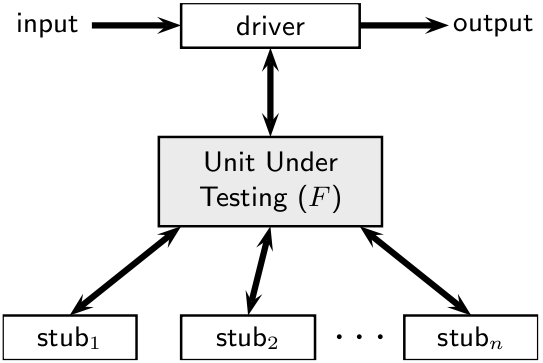
\includegraphics[scale=.3]{teste-de-software/conceitos-basicos/Imagens/driver-e-stub}
\end{block:fact}
\end{frame}



\begin{frame}
\label{concept:teste-de-integracao}
\frametitle{Fases de teste}
\framesubtitle{Teste de integração}

\begin{block:concept}{Definição}
Teste de integridade verifica se as variáveis testadas individualmente se comunicam corretamente quando integrado.
\end{block:concept}

\begin{block:fact}{}
    \centering
    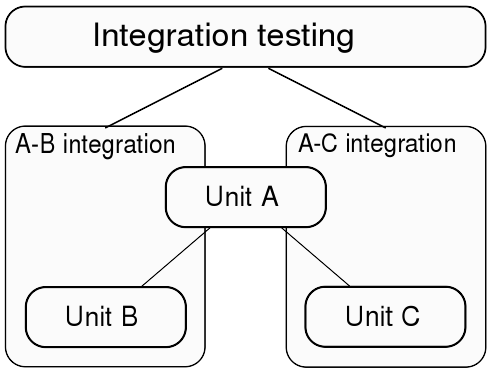
\includegraphics[scale=.3]{teste-de-software/conceitos-basicos/Imagens/integration-testing}
\end{block:fact}

\hfill
\refie{example:mars-climate-orbiter}{\beamerbutton{Example: Mars climate orbiter}}
\end{frame}



\begin{frame}
\frametitle{Fases de teste}
\framesubtitle{Teste de integridade}

\begin{block:fact}{Por que o teste de integração é importante?}
\begin{itemize}
	\item Teste de integridade deve ser executado porque:
	\begin{itemize}
		\item Os dados podem ser perdidos na interfáce da variável;

		\item Variáveis globais podem sofrer interferências indesejadas.
	\end{itemize}
\end{itemize}
\end{block:fact}

\begin{block:fact}{}
    \centering
    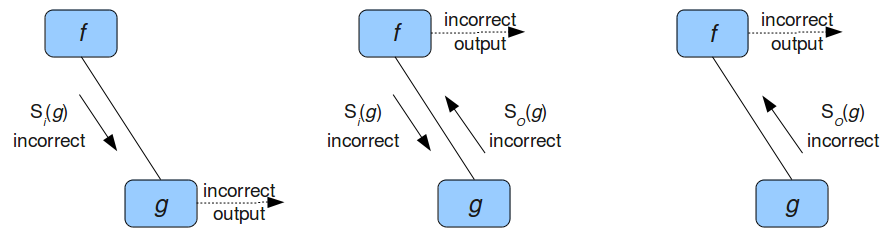
\includegraphics[width=\textwidth]{teste-de-software/conceitos-basicos/Imagens/types-integration-errors}
\end{block:fact}
\end{frame}


\begin{frame}
\label{concept:system-testing}
\frametitle{Fases de teste}
\framesubtitle{Teste de sistema}

\begin{block:concept}{Definição}
Teste de sistema garante que o software e os outros elementos que fazem parte do sistema (hardware e banco de dados, por exempo) são combinados adequadamente e se comportam conforme o esperado.
\end{block:concept}

\begin{block:fact}{Tipos de teste de sistema}
\begin{itemize}
	\item Normalmente o teste de sistema inclui muitos tipos de teste
	\begin{columns}[t, totalwidth=6.5cm]
		\begin{column}[t]{3cm}
			\begin{itemize}
				\item Funcionalidade;,
				\item Usabilidade;
				\item Segurança;
				\item Localização.
			\end{itemize}
		\end{column}

		\begin{column}[t]{3cm}
			\begin{itemize}
				\item Confiabilidade;
				\item Disponibilidade.
				\item \ldots
			\end{itemize}
		\end{column}
	\end{columns}
\end{itemize}
\end{block:fact}

\hfill
\refie{example:trem-fantasma}{\beamerbutton{Example: Trem fantasma}}
\end{frame}



\begin{frame}[hasprev=true, hasnext=false]
\label{concept:acceptance-testing}
\frametitle{Fases de teste}
\framesubtitle{Teste de aceitação}

\begin{block:concept}{Definição}
Teste de aceitação refere-se ao avaliador, geralmente realizado pelo próprio usuário que verifica se o produto satisfaz sua expectativa.
\end{block:concept}

\begin{block:fact}{Teste Alfa/Beta}
\begin{itemize}
	\item Informalmente, pode ser definido como teste alfa e beta:
	\begin{itemize}
		\item Teste alfa: o software é instalado e usado internamente (na em presa em que foi desenvolvida);

		\item Teste beta: o software é instalado e testado por usuários exeternos.
	\end{itemize}
\end{itemize}
\end{block:fact}

\begin{block:fact}{Por que o teste de aceitação é importante?}
\begin{itemize}
    \item O teste de aceitação, quando concluído com sucesso, resultará na aceitação do software pelo cliente.
\end{itemize}
\end{block:fact}
\end{frame}